\documentclass[11pt]{article}
\usepackage[margin=1in]{geometry}
\usepackage{amsmath,amssymb,amsthm}
\usepackage{graphicx}
\usepackage{enumitem}
\usepackage[hidelinks]{hyperref}
\usepackage{caption}
\usepackage{booktabs}
\captionsetup{font=small,labelfont=bf}

\newtheorem{theorem}{Theorem}
\newtheorem{lemma}{Lemma}
\newtheorem{proposition}{Proposition}
\newtheorem{corollary}{Corollary}
\theoremstyle{definition}
\newtheorem{definition}{Definition}
\newtheorem{remark}{Remark}

\newcommand{\Z}{\mathcal{Z}}
\newcommand{\X}[1]{X_{#1}}

\title{\vspace{-1.2em}Locality of $\mathrm{Tr}(\phi^3)$ tree amplitudes from cyclic hidden zeros\\[2pt]
\large Part II: the fat--zero generalisation}
\date{}
\author{}

\begin{document}
\maketitle
\vspace{-3.2em}

\begin{abstract}
\noindent We promote the hidden $1$--zero to a \emph{$k$--zero} (``fat zero''): the simultaneous
imposition of the hidden--zero relations on $k$ consecutive boundaries. A $k$--zero kills strictly
more nonlocal coefficients than the $1$--zero, with a clean geometric criterion. For every $k$
consecutive edges of the $n$--gon, the $(k{+}1)$--gon $N$ spanned by those edges must either
\emph{(P2)} extend to a $(k{+}2)$--gon built from chords of the diagram, or \emph{(P1)} contain a
chord crossing the enclosing chord. The $(k{+}2)$--gons completing successive $k$--zeros build on
top of each other: the $(k{+}2)$--gon at the $k$--zero is itself the $(k{+}1)$--gon at the next
$(k{+}1)$--zero, so the family stacks. Under (P1) the chord identities couple the surviving chord
with a \emph{partner} that must scale with the special chord, forcing every $(k\ge 1)$ survivor to
contain at least two chords in an incompatible pairing. Across all $k$ and all cyclic rotations, the
union of these conditions is satisfied exactly by the triangulations (conjecturally; verified at
$n\le 7$ via a direct rank computation). The Step--$2$ coefficient equations are in Part~III.
\end{abstract}

\section{From one zero to many}
We keep the conventions of Part~I. The $n$-gon has vertices $1,\dots,n$; a chord $\X{ij}$
($1\le i<j\le n$, $|j-i|\neq 1$, $(i,j)\neq(1,n)$) is a variable; an edge $\X{m,m+1}$ is a leg and
equals~$0$. The ansatz is $B_n=\sum_{|M|=n-3}a_M\big/\!\prod_{c\in M}\X{c}$ over multisets $M$, and
locality is the statement $a_M=0$ whenever $M$ contains a crossing pair.

A cyclic hidden \emph{$1$--zero} imposes the $n-3$ relations $c_{1j}=0$, where
\begin{equation}\label{eq:c}
  c_{ij}=\X{ij}+\X{i+1,\,j+1}-\X{i,\,j+1}-\X{i+1,\,j}.
\end{equation}
On $\Z_{1,3}$ these read $\X{2k}=\X{1k}-\X{13}$ and $\X{2n}=-\X{13}$; the \emph{special} chord is
$\X{13}$ and the \emph{bare} chord is $\X{2n}$.

\begin{definition}[$k$--zero]\label{def:kzero}
For $1\le k\le n-3$, the \emph{$k$--zero based at $\{1,\dots,k{+}1\}$} is the simultaneous imposition
\begin{equation}\label{eq:kzero}
  c_{ij}=0,\qquad i=1,\dots,k,\quad j=k+2,\dots,n-1 .
\end{equation}
\end{definition}
\noindent It collects the hidden--zero relations on the $k$ consecutive boundaries
$(1,2),(2,3),\dots,(k,k{+}1)$. For $k=1$ it is the ordinary $1$--zero. There are $k(n-k-2)$ relations
and they cut out a linear surface $\Z^{(k)}$.

\section{The constraint surface of a $k$--zero}
\begin{lemma}[Telescoping]\label{lem:tele}
On $\Z^{(k)}$, with the leg convention $\X{m,m+1}=0$,
\begin{align}
  \X{k+1,\,j} &= \X{1j}-\X{1,k+2}, & j&=k+3,\dots,n-1; & \X{k+1,\,n}&=-\X{1,k+2},\label{eq:backbone}\\
  \X{ij} &= \X{k+1,\,j}+\X{i,\,k+2}, & i&=2,\dots,k,\ \ j=k+3,\dots,n.\label{eq:interior}
\end{align}
\end{lemma}
\begin{proof}
Sum \eqref{eq:c} over the full block of rows $i=1,\dots,k$ at fixed $j$. The two inner sums
telescope, leaving $\sum_{i=1}^{k}c_{ij}=\bigl(\X{1j}-\X{k+1,j}\bigr)-\bigl(\X{1,j+1}-\X{k+1,j+1}\bigr)=0$,
so $\X{k+1,j}-\X{1j}$ is independent of $j$; evaluating at $j=k+2$ (with $\X{k+1,k+2}=0$) gives
\eqref{eq:backbone}, and at $j=n$ (with $\X{1n}=0$) the bare relation. Summing the partial block
$i'=i,\dots,k$ gives $\X{ij}-\X{i,j+1}=\X{k+1,j}-\X{k+1,j+1}$; telescoping in $j$ from $k+2$ yields
\eqref{eq:interior}.
\end{proof}

\noindent Three structures organise $\Z^{(k)}$ (Figure~\ref{fig:geometry}).
\begin{itemize}[topsep=2pt,itemsep=1pt]
  \item The \textbf{near block} $N=\{1,\dots,k{+}1\}$ and the \textbf{far block}
  $F=\{k{+}2,\dots,n\}$. Every chord internal to $N$ or to $F$ is absent from \eqref{eq:kzero}:
  these are the \emph{born--free} chords, untouched by the $k$--zero.
  \item The length--$k$ \textbf{enclosing chord} $\X{1,k+1}$ closes the $k$ consecutive boundaries
  into the $(k{+}1)$--gon $N$. It is itself born--free.
  \item The \textbf{special} $\X{1,k+2}$ and the \textbf{bare} $\X{k+1,n}$ --- exact analogues of
  $\X{13}$ and $\X{2n}$ at $k=1$ --- each bridge $N$ to $F$ across one boundary of $N$.
\end{itemize}
The remaining bridges between $N$ and $F$ organise into \emph{columns}: for each far vertex
$\ell\in F$, the column at $\ell$ is the tuple
$\bigl(\X{1\ell},\X{2\ell},\dots,\X{k+1,\ell}\bigr)$ of $k{+}1$ chords. Equations
\eqref{eq:backbone}--\eqref{eq:interior} couple these together.

\begin{figure}[t]
  \centering
  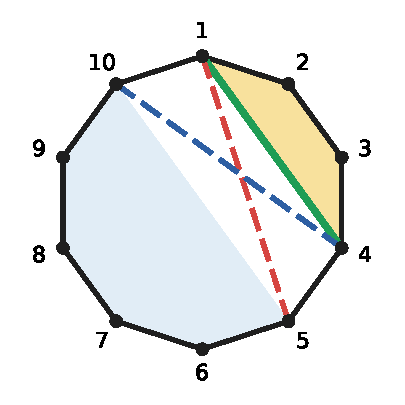
\includegraphics[width=0.36\textwidth]{figures/geometry.pdf}
  \caption{Geometry of a $k$--zero ($n=10$, $k=3$). Near block $N=\{1,2,3,4\}$ (gold); far block
  $F=\{5,\dots,10\}$ (blue). Green: the length--$k$ enclosing chord $\X{1,4}$. Red dashed: special
  $\X{1,5}$. Blue dashed: bare $\X{4,10}$.}
  \label{fig:geometry}
\end{figure}

\section{The geometric survival theorem}\label{sec:survival}
The kill mechanism is the Laurent argument: take an asymptotic limit on $\Z^{(k)}$ in which the
special chord diverges; the multisets whose chords \emph{all} stay finite form a vanishing
polynomial in the finite coordinates, forcing $a_M=0$ on every such $M$. Running the argument with
every admissible limit produces a single geometric criterion.

\begin{theorem}[Survival]\label{thm:survival}
Fix $k\in\{1,\dots,n{-}3\}$ and the $k$--zero based at the $(k{+}1)$--gon $N=\{i,\dots,i{+}k\}$
with enclosing chord $\X{i,i+k}$. A multiset $M$ survives this $k$--zero iff at least one of:
\begin{description}[topsep=2pt,itemsep=2pt,leftmargin=2.4em]
  \item[\textnormal{(P1)}] $M$ contains a chord that crosses $\X{i,i+k}$, i.e.\ a chord with one
  endpoint strictly inside $N$ and one strictly outside.
  \item[\textnormal{(P2)}] $M$ extends $N$ to a $(k{+}2)$--gon, i.e.\ $M$ contains chords
  completing $\{i,\dots,i{+}k,v\}$ as a polygon, for some far vertex $v\in F$.
\end{description}
\end{theorem}

\noindent The next sections unpack (P2) (the easy half) and (P1) (where the real content lives).

\section{P2: $(k{+}2)$--gons over $(k{+}1)$--gons, stacking}\label{sec:kp2}
For $v\in F=\{k{+}2,\dots,n\}$, the $(k{+}2)$--gon $\{1,\dots,k{+}1,v\}$ is closed in the polygon by
exactly one of three configurations (Figure~\ref{fig:kgon}):
\begin{enumerate}[label=(\roman*),topsep=2pt,itemsep=1pt]
  \item $v=k{+}2$: the edge $(k{+}1,k{+}2)$ + the chord $\X{1,k+2}$ -- the \textbf{special}.
  \item $v=n$:    the edge $(n,1)$       + the chord $\X{k+1,n}$ -- the \textbf{bare}.
  \item $v\in\{k{+}3,\dots,n{-}1\}$: two chords $\X{1,v}$ and $\X{k+1,v}$ -- the \textbf{column pair}.
\end{enumerate}
\begin{figure}[t]
  \centering
  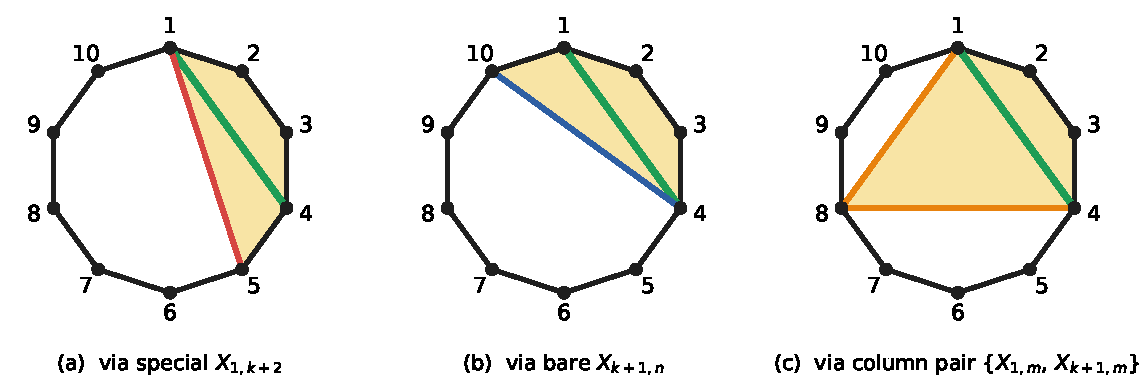
\includegraphics[width=0.95\textwidth]{figures/kplus2gon.pdf}
  \caption{The three $(k{+}2)$--gon completions of $N$ ($n=10$, $k=3$, $m=8$ for the column pair).}
  \label{fig:kgon}
\end{figure}

\paragraph{Stacking.}
The $(k{+}2)$--gon that closes a survival at the $k$--zero is itself the $(k{+}1)$--gon at the
$(k{+}1)$--zero based at the same vertex, which in turn must extend to a $(k{+}3)$--gon, and so on
(Figure~\ref{fig:stack}). The family of $k$--zero survival conditions therefore \emph{stacks}: each
step adds one more vertex to the enclosing polygon.
\begin{figure}[h]
  \centering
  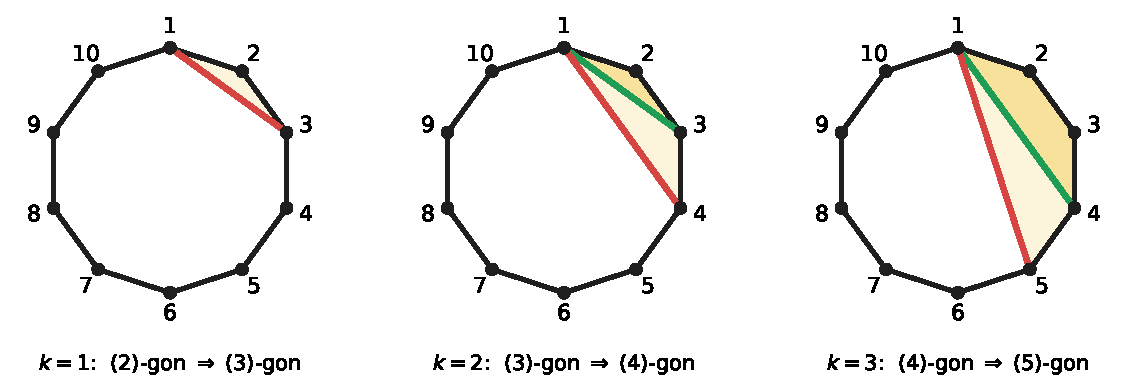
\includegraphics[width=0.95\textwidth]{figures/stacking.pdf}
  \caption{Stacking ($n=10$). The $(k{+}2)$--gon over $k$ edges (lighter shading) is the
  $(k{+}1)$--gon at the next step. Triangle $\Rightarrow$ $4$--gon $\Rightarrow$ $5$--gon $\Rightarrow\cdots$\,.}
  \label{fig:stack}
\end{figure}

\section{P1: the partner--chord forcing}\label{sec:p1}
The interesting content of Theorem~\ref{thm:survival} is the P1 case. To explain what survival
requires concretely, we follow the asymptotic analysis of notes~24--25: the chord identities
\eqref{eq:backbone}--\eqref{eq:interior} couple the bridges so tightly that holding a single chord
finite under the kill limit \emph{forces} other chords to grow along with the special. Survival
then requires two chords whose forced behaviours conflict.

\paragraph{Setup.}
Write the special as $s=\X{1,k+2}$ and take $s\to\infty$. By \eqref{eq:backbone}--\eqref{eq:interior},
every constrained chord can be written in terms of $s$, the column-$(k{+}2)$ offsets
$t_i:=\X{i,k+2}\ (i=2,\dots,k)$, and the column-$1$ values $u_\ell:=\X{1\ell}\ (\ell=k{+}3,\dots,n{-}1)$:
\begin{equation}\label{eq:column-formulas}
  \X{1,\ell}=u_\ell,\qquad
  \X{k+1,\ell}=u_\ell-s,\qquad
  \X{i,\ell}=u_\ell-s+t_i\ (2\le i\le k),
\end{equation}
together with $\X{i,n}=t_i-s$ and the bare $\X{k+1,n}=-s$. As $s\to\infty$, each finite-or-not
status of a chord is dictated by whether \emph{combinations} of $s,u_\ell,t_i$ cancel.

\paragraph{Partner forcing.}
For each chord, the requirement that it stay finite forces particular other chords to grow with $s$
(``partners''):
\begin{center}\small
\begin{tabular}{lll}
\toprule
chord finite & forced behaviour & geometric reading\\
\midrule
$\X{1,\ell}$            & $u_\ell$ stays finite                 & ``$1$--side'' of column $\ell$ \\
$\X{k+1,\ell}$          & $u_\ell$ grows with $s$               & ``$(k{+}1)$--side'' of column $\ell$ \\
$\X{i,\ell}$ (interior) & $u_\ell+t_i$ grows with $s$           & needs offset $t_i$ to compensate \\
$\X{i,k+2}$ (offset)    & $t_i$ stays finite                    & column-$(k{+}2)$ offset on the $1$--side \\
$\X{i,n}$ (offset-$n$)  & $t_i$ grows with $s$                  & column-$(k{+}2)$ offset on the $(k{+}1)$--side \\
\bottomrule
\end{tabular}
\end{center}
The \emph{special} and \emph{bare} themselves are bare powers of $\pm s$ and are never finite.

\paragraph{Why ``two chords always''.}
Holding a \emph{single} chord finite never produces a contradiction --- there is always some choice
of rates for the other coordinates that makes it work. A multiset survives the kill iff it contains
\emph{at least two chords} whose finite-requirements are mutually incompatible. The cleanest such
incompatibilities are:
\begin{enumerate}[label=(\textsc{p\arabic*}),topsep=2pt,itemsep=1pt]
  \item \textbf{Column pair} $\{\X{1,\ell},\X{k+1,\ell}\}$ at the same $\ell$:
        forces $u_\ell$ both finite (from the first chord) and growing with $s$ (from the second).
        Impossible.
  \item \textbf{Offset pair} $\{\X{i,k+2},\X{i,n}\}$ at the same $i$:
        forces $t_i$ both finite and growing with $s$. Impossible.
  \item \textbf{Special--anything} or \textbf{bare--anything}: the special or bare alone already
        cannot be held finite, so any multiset containing one survives.
\end{enumerate}
Geometrically, (\textsc{p1})--(\textsc{p3}) are exactly the $(k{+}2)$--gon completions of
Section~\ref{sec:kp2}. The chord identities turn each $(k{+}2)$--gon completion into a
partner--chord pair, and conversely each incompatible chord pair completes a $(k{+}2)$--gon.
\emph{The same two chords appear in both readings.}

\paragraph{Worked example ($k=2$).}
For the $2$--zero based at $\{1,2,3\}$, $\X{3\ell}=\X{1\ell}-\X{14}$ and
$\X{2\ell}=\X{1\ell}-\X{14}+\X{24}$. Take $\X{14}=s\to\infty$.
\begin{itemize}[topsep=2pt,itemsep=1pt]
  \item Single chord $\X{2,5}\in M$: the identity $\X{2,5}=\X{1,5}-s+\X{2,4}$ stays finite if either
  $\X{1,5}$ grows with $s$ (and $\X{2,4}$ stays finite), or $\X{2,4}$ grows with $s$ (and
  $\X{1,5}$ stays finite). One of the two suffices, so $M$ is killed.
  \item Pair $\{\X{1,5},\X{3,5}\}\in M$: $\X{3,5}=\X{1,5}-s$ stays finite iff $\X{1,5}$ grows with
  $s$. But then $\X{1,5}$ itself cannot stay finite. Contradiction. $M$ survives.
  \item Pair $\{\X{2,4},\X{2,7}\}\in M$ (here $n=7$): $\X{2,7}=\X{2,4}-s$ finite iff $\X{2,4}$ grows
  with $s$, but $\X{2,4}$ alone forces itself finite. Contradiction. $M$ survives.
\end{itemize}
The pattern is general: surviving a $k$--zero via the P1 mechanism always means hitting one of the
incompatible pairs above. \emph{Survival is a pairing condition, not a single-chord condition.}

\section{The per--column choice}\label{sec:column}
The partner-forcing rules in Section~\ref{sec:p1} can be summarised cleanly per column. Fix a far
vertex $\ell\in\{k{+}3,\dots,n{-}1\}$. The $k{+}1$ chords of column $\ell$ are
$\X{1,\ell},\,\X{2,\ell},\dots,\,\X{k,\ell},\,\X{k+1,\ell}$. By \eqref{eq:column-formulas} they are
locked together: \emph{at most one of three exclusive ``slots'' per column can be held finite}
(Figure~\ref{fig:column}):
\begin{enumerate}[label=(\roman*),topsep=2pt,itemsep=1pt]
  \item the \textbf{$1$--slot} $\{\X{1,\ell}\}$ alone;
  \item the \textbf{$(k{+}1)$--slot} $\{\X{k+1,\ell}\}$ alone;
  \item the \textbf{interior slot} $\{\X{2,\ell},\dots,\X{k,\ell}\}$ (here $u_\ell-s$ is the same for
        every entry, so they all become finite or all infinite together).
\end{enumerate}
\begin{figure}[t]
  \centering
  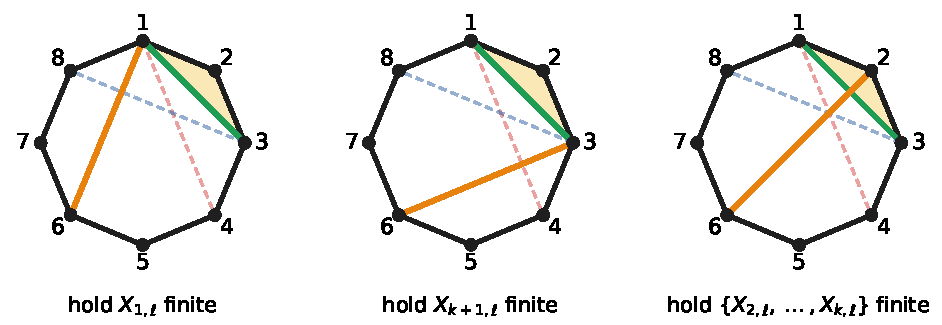
\includegraphics[width=0.93\textwidth]{figures/column_rule.pdf}
  \caption{The per--column slots at $\ell$ ($n=8$, $k=2$). Per column we can hold one of the three
  slots finite. A multiset is killed iff at every far column its chords fit inside one slot.}
  \label{fig:column}
\end{figure}

\noindent Two more choices govern the boundary columns: at column $k{+}2$ the offsets
$\{\X{i,k+2}:2\le i\le k\}$ are held finite together (``$1$--side''); at column $n$ the offsets
$\{\X{i,n}:2\le i\le k\}$ are held finite together (``$(k{+}1)$--side''); these two are mutually
exclusive. The column pair $\{\X{1,\ell},\X{k+1,\ell}\}$ and the offset pair
$\{\X{i,k+2},\X{i,n}\}$ are exactly the violations of these exclusivities.

\section{P1 across all $k$: many crossings at once}\label{sec:fan}
From a single base vertex $i$, the enclosing chords of the successive $k$--zeros form a fan,
$$\{\X{i,i+2},\ \X{i,i+3},\ \dots,\ \X{i,\,i+\lfloor n/2\rfloor}\},$$
shown in Figure~\ref{fig:fan}. A multiset that
survives \emph{every} such $k$--zero by the P1 mechanism alone --- never closing a $(k{+}2)$--gon
--- must contain a chord crossing each enclosing chord in the fan. So $M$ needs $\sim n/2$ chords
covering the entire fan simultaneously, and by the partner forcing of Section~\ref{sec:p1} each
crossing brings its own partner. Including cyclic rotations the count scales like $n^2/4$, severely
restricting the multiset shape.
\begin{figure}[h]
  \centering
  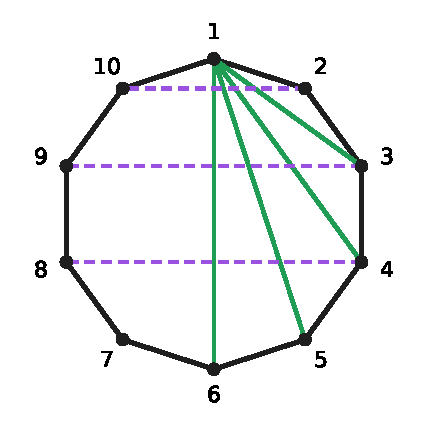
\includegraphics[width=0.30\textwidth]{figures/fan.pdf}
  \caption{Fan of enclosing chords from vertex $1$ at $n=10$ (green). Each $k$--zero based at vertex
  $1$ has its own enclosing chord; surviving the family by P1 alone requires a chord crossing each
  of them (purple dashed = sample crossings).}
  \label{fig:fan}
\end{figure}

\section{Survivors: a worked gallery}\label{sec:gallery}
At $n=7$ on the $k=2$ zero based at $\{1,2,3\}$, a multiset has $n-3=4$ chords. Survival means $M$
contains the special, the bare, a column pair, or an offset pair (Figure~\ref{fig:gallery}). Each
panel shows a concrete surviving multiset; the highlighted pair is the structural reason for
survival, and the other chords are filler from the born--free set (which is always finite and so
contributes nothing to the kill).

\begin{figure}[h]
  \centering
  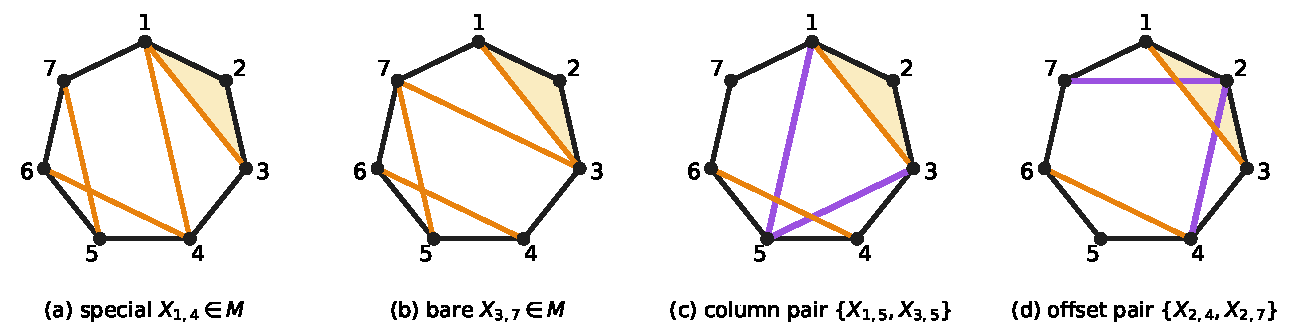
\includegraphics[width=0.95\textwidth]{figures/survivor_gallery.pdf}
  \caption{Four surviving multisets on the $k=2$ zero, $n=7$. (a)(b) the special and the bare cases
  (the geometric $(k{+}2)$--gon completion fires). (c) the column pair $\{\X{1,5},\X{3,5}\}$ forces
  $u_5$ to be both finite and divergent. (d) the offset pair $\{\X{2,4},\X{2,7}\}$ forces $t_2$ to
  be both finite and divergent. The same multisets are listed in the asymptotic case analysis of
  note~25 (page~3, top row).}
  \label{fig:gallery}
\end{figure}

\noindent Survivors at higher $k$ have the same shape: each contains at least one column pair, one
offset pair, the special, or the bare, possibly with additional crossings layered on top.

\section{Triangulations escape}\label{sec:triangs}
\begin{proposition}\label{prop:tri-escape}
Every triangulation of the $n$--gon satisfies Theorem~\ref{thm:survival} at every $k$ and every
cyclic rotation.
\end{proposition}
\begin{proof}
Fix $k$ consecutive edges. If no chord of the triangulation crosses the enclosing chord
$\X{1,k+1}$, then adjoining $\X{1,k+1}$ crosses nothing, so it is already in the triangulation; being
a triangulation chord, it bounds a triangle on its far side, extending $N$ to a $(k{+}2)$--gon
(P2). Otherwise (P1).
\end{proof}

\begin{quote}
\textbf{Conjecture (all--$n$ locality).} The union of the $k$--zero survival conditions across all
$k$ and all cyclic rotations is satisfied exactly by the triangulations of the $n$--gon.
\end{quote}
\noindent At $n\le 9$ this is proven by direct enumeration in Part~I, and at $n\le 7$ it is
verified end--to--end by the rank computation in
\texttt{computations/full\_constraint\_system/}: the full constraint matrix has rank $T(n)-1$,
with kernel spanned exactly by the triangulation indicator.

\section{Status}\label{sec:status}
Theorem~\ref{thm:survival} gives the geometric kill criterion. The substantive content is the
partner-forcing of Section~\ref{sec:p1}: holding one chord finite forces its partner to scale with
the special, so survival is always a pairing condition. The per-column choice
(Section~\ref{sec:column}) compiles this into one slot per far vertex, and the fan argument
(Section~\ref{sec:fan}) shows that escaping by P1 alone requires $\sim n/2$ simultaneous crossings.
Triangulations are the only multisets known to satisfy all conditions; the all--$n$ converse
requires reading the conditions together with the Step--$2$ coefficient equations of Part~III,
which fix the relative values of the surviving coefficients.

\end{document}
